\chapter{Programmierhandbuch}

    \section{Entwicklungskonfiguration}
        Das Programm \textit{Scotland Yard} wurde mit hilfe folgenden Komponenten entwickelt.
        \begin{table}[H]
            \caption{Programmanforderung}
            \begin{tabular}{p{6cm}  p{6cm}} 
                \hline
                \textbf{Software} & \textbf{Version}\\
                \hline
                Betriebssystem & Manjaro Linux - Kernel 5.3.18\\
                Java Development KIt & OpenJDK 1.8\\
                JavaFX & 8.0\\
                Software zur Erstellung der GUI &  Scene Builder 8.4.1\\
                IDE & Netbeans 8.2\\
                \hline
            \end{tabular}
        \end{table}

    \newpage
    \section{Problemanalyse und Realisation}
        In diesem Abschnitt werden Probleme aus der Aufgabenstellung analysiert, die daraus resultierenden
        Überlegungen dargestellt und die finalen gewählten Lösungen begründet.

        \subsection{Spielfeld}\label{gameboard}

            Das Spielfeld von \textit{Scotland Yard} besteht aus 199 Stationen die jeweils über Verkehrsmittel verbunden sind.
            Dabei gibt es Taxi-, Bus-, U-Bahn- und Bootsverbindungen.
            In diesem Netz können sich die Spieler mit Hilfe ihrer Verkehrestickets bewegen.
            
            \subsubsection{Parsen des Spielfeldes}

                Das Spielfeld welches durch die Aufgabenstellung vorgegeben ist und in einer JSON-Datei abgelegt ist,
                wird für jeden Programmstart benötigt. Durch parsen der JSON-Datenstruktur werden benötigte Spielfeldinformationen
                extrahiert und in interne Repräsentationen übersetzt.
                Dabei besteht die JSON-Datenstruktur aus mehreren Stationen die unterneinader durch die Verkehrsmittel verbunden sind.
                Jede Station besitz zusätzlich eine eindeutige Identifikationsnummer und eine Position aus X- und Y-Koordinaten.
                \newline
                Der Vorgang des parsen wird über eine Bibliothek namens \textit{GSON} realisiert.
                Diese ermöglicht es die JSON-Datenstruktur ähnlich wie einen Baum zu durchlaufen
                oder komplette Strukturen direkt in eine interne Repräsentation zu übersetzen.
                \newline
                \newline
                Durch die jeweilige Verbindungen der Stationen unterneinader entsteht eine Netzstruktur.

                Der erste Ansatz ist die JSON-Datenstruktur zu durchlaufen und
                die Stationen direkt zu erstellen und diese über ihre Identifikationsnummer zu Verknüpfen.
                Der Vorteil hierbei ist, dass die JSON-Datenstruktur nur einmal durchlaufen werden muss.
                Ein offensichtlicher Nachteil ist jedoch, dass das Netz nicht ohne die dahinter liegende
                interne Struktur durlaufen werden kann.
                Das heißt, dass von einer Station nicht direkt auf eine andere referenziert werden kann.

                Ein anderer Ansatz ist es, die interne Repräsentation so aufzubauen,
                dass eine Station direkt auf all ihre Nachbarn zeigt.
                Auf der einen Seite ist somit sichergestellt, dass von jeder Station aus das ganze Netz durlaufen werden kann.
                Auf der anderen Seite muss nun die Json-Datenstruktur zweimal durchlaufen werden.
                Einmal um alle Stationen und somit ihre Referenzen zu erstellen.
                Das zweite Mal um die Stationen miteinander zu verbinden.

                Obwohl der zweite Ansatz das parsen der JSON-Datenstruktur komplexer macht, 
                wurde dieser, für die interne Repräsentation des Spielfeldes,
                gewählt da somit alle Operationen auf dem Netz enorm vereinfacht werden.
                \newline
                \newline
                Nach dem Parsen hält die Klasse \textit{Board} nun alle Stationen in einer \textit{ArrayList}.
                Somit kann effizient, mit hilfe der Identifikationsnummer einer Station, indiziert auf eine Station zugegriffen werden.

            \paragraph{Validieren der Datenstruktur}\label{validate}
                
                Da beim Parsen der \textit{JSON}-Datenstruktur Fehler auftretten können, muss diese zunächst validiert werden.
                Dabei wird zwischen Speicherstrukturfehlern, die also die formale Korrektheit des \textit{JSON}-Formats betreffen und
                den inhaltlichen Fehlern, die sich in ungültigen Werten wiederspiegeln, unterschieden.
                Die \textit{GSON}-Bibliothek fängt dabei die formalen Fehler ab und schmeißt in solch einem Fall eine \textit{JsonSyntaxException}.
                Die statischen Methoden der \textit{JsonValidator}-Klasse überprüfen hingegen die Korrektheit der inhaltlichen Struktur und schmeißt
                eine \textit{IllegalArgumentException} falls ein Feld oder der Datentyp des Feldes falsch ist.
                \newline
                Um ein fehlerhaftes Spielfeld zu unterbinden wird zusätzlich geprüft, ob die verknüpften Stationen auch wirklich existieren.
                Dabei wird im Fehlerfall eine \textit{IllegalArgumentException} geworfen.
                
            \subsubsection{Stationen}\label{stations}
                Die Stationen sind als Knotenpunkte und deren Verbindungen als Kanten innerhalb des Netzes zu sehen.
                Da eine Station somit auf all ihre direkten Nachbarn referenziert, kann von einer Station, über Zwischentationen,
                jede andere Station erreicht werden.
                
                \paragraph{Occupied-Flag}
                    Eine Station bietet jedoch immer nur Platz für einen Spieler.
                    Daraus folgt, dass eine Station besetzt sein kann und dass kein anderer Spieler die Verbindungen der besetzen Stationen nutzen kann.
                    Dies wird über ein boolesches Flag (\textit{Occupied}-Flag) innerhalb der \textit{Station}-Klasse erreicht.
                    Somit ist die information ob eine Station besetzt ist, in dem Netz enthalten.

                    Dies hat den Vorteil, dass ein Spieler die anderen Spielerpositionen nicht kennen muss um sich Regelkonform durch das Netz zu bewegen.
                    Daraus folgt auch, dass jeder Spieler der auf eine Station ziehen möchte, zunächst das Flag testen muss.
                    Zusätzlich muss jeder Spieler nach jedem erfolgreichen Zug das Flag in der Zielstation auf \textit{true} und in der verlassenen Station
                    auf \textit{false} setzen.
                    Zieht jedoch ein Spieler auf eine besetzte Station und versucht das \textit{Occupied}-Flag zu setzen, wird eine \textit{IllegalStateException}
                    geworfen. Somit können Programmierfehler leicht erkannt werden.

                \paragraph{Traversieren des Netzes}
                    Da die \textit{Station}-Klasse zuständig ist, um sich durch das Netz zu bewegen bzw. Nachbarstationen zu erhalten,
                    spielt diese eine große Rolle für viele Algorithmen.
                    Deshalb wurden grundsätzlich zwei Verfahren gewählt um sich durch das Netz zu bewegen.
                    \newline
                    Die eine Methode \textit{getStationsReachableBy} gibt alle Stationen wieder die über ein bestimmtes Ticket erreichbar sind.
                    Falls keine Station über dieses Ticket erreichbar ist, wird ein leeres \textit{Set} zurück gegeben.
                    \newline
                    \newline
                    \texttt{Set<Station> getStationsReachableBy(Ticket ticket)}
                    \newline
                    \newline
                    Dabei ist zu beachten, dass aus der Aufgabenstellung hervorgeht, dass das \textit{Blackticket} ein Allzweckticket ist.
                    Somit werden alle Nachbarstationen zurück gegeben falls diese Methode mit dem \textit{Blackticket} aufgerufen wird.
                    \newline
                    Die andere Methode \textit{getTicketsToReachableStation} gibt das Ticket wieder welches benötigt wird um sich zu einer bestimmten Station zu bewegen.
                    Falls die übergebene Station nicht über die Verbindungen dieser Station erreichbar ist, wird ein leeres \textit{Set} zurück gegeben.
                    \newline
                    \newline
                    \texttt{Set<Ticket> getTicketsToReachableStation(Station station)}
                    \newline
                    \newline
                    Auch hierbei ist zu beachten, dass das \textit{Blackticket} jedes Mal mit zurückgegeben wird sobald die
                    übergebenen Station eine Nachbarstation ist.
 
        \subsection{Spieler}

            Das wohl wichtigste Spielelement ist der Spieler und seine Funktionen sich durch das Netz zu bewegen.
            Dabei wird zwischen Mister-X und einem Detektiv als Spielertypen unterschieden.
            Jeder der beiden Typen nutzt dabei allgemeine aber auch spezialisierte Methoden um am Spielgeschehen teilzunehmen.
            
            \subsubsection{Obertyp}
                Allgemeine Funktionen wie die Ticketverwaltung, die Position, sowie die Bewegung durch das Netz und einige KI-Anteile sind
                in einem abstrakten Obertypen namens \textit{Player} zusammengefasst.
                Dadurch lässt sich ein allgemeiner Spielertyp modellieren und Spezialisierungen in den jeweiligen Unterklassen formulieren.
                \newline
                \newline
                \paragraph{Ticket}
                    Da alle Spieler Tickets brauchen um sich durch das Netz zu bewegen, sind diese sowie ihre Verwaltung innerhalb
                    der Oberklasse angesiedelt. Konkret ist ein Ticket ein \textit{Enum} und besteht aus den Werten
                    \textit{CAB}, \textit{BUS}, \textit{TUBE} und \textit{BLACK}.
                    Nun gibt es mehrere Ansätze die Tickets zu speichern und den Zugriff auf diese zu realisieren.
                    \newline
                    Ein Ansatz wäre es für jede Ticketart eine eigene Variable zu benutzen.
                    Dies verkompliziert jedoch den Zugriff auf die Tickets massiv, da jeder Zugriff in langen \textit{Switch}-Konstrukten resultiert.
                    Zusätzlich muss für jedes neue Ticket ein \textit{Switch-Case}, in jeder Methode die die Tickets verarbeitet hinzugefügt werden.
                    \newline
                    Ein alternativer Ansatz wäre es die Tickets in einem \textit{Array} zu speichern.
                    Dies hat den Vorteil, dass direkt über den Ordinalwert des Ticketenums, indiziert auf das \textit{Array} zugegriffen werden kann.
                    Neu hinzugefügte Tickets sind somit wartbarer.
                    \newline
                    Somit kann das Array dynamisch aus den Tickets konstruiert werden.
                    \newline
                    \newline
                    \texttt{new int[Ticket.values().length]}
                    \newline
                    \newline
                    Aus diesen Gründen wurde für die Implementierung der Tickets der zweite Ansatz gewählt.

                \paragraph{Aktuelle Position}
                    Jeder Spieler hält seine aktuelle Position, das heißt die Station auf der er sich befindet.
                    Somit hat jeder Spieler einen Einstiegspunkt in das Netz. Alle Methoden wie z.B. die Überprüfung ob eine Station erreichbar is
                    oder welche Tickets benötigt werden um eine Station zu erreichen, arbeiten somit direkt mit diesem Einstiegspunkt.

                \paragraph{Erreichbare Stationen}
                    Eine grundsätzliche und für fast alle Algorithmen wiederkehrende Problematik ist das Bestimmen der erreichbaren Stationen.
                    Eine erreichbare Station ist jene, die über eine Verbindung der aktuellen Station erreichbar ist.
                    Als Einschränkungen müssen jedoch das \textit{Occupied}-Flag und die verfügbaren Tickets beachtet werden.
                    Um alle erreichbaren Stationen eines Spielers zu bekommen, kann somit auf die \textit{getReachableStations}-Methode
                    zurückgegriffen werden.

                    \begin{lstlisting}
public Set<Station> getReachableStations() {
    return Arrays.stream(Ticket.values())
    .filter(ticket -> this.getTicketNum(ticket) > 0)
    .map(ticket -> this.currentStation.getStationsReachableBy(ticket))
    .flatMap(Collection::stream)
    .distinct()
    .filter(station -> !station.isOccupied())
    .collect(Collectors.toCollection(HashSet::new));
}
                    \end{lstlisting}
                    Dabei wird zunächst ein \textit{Stream} aus allen Tickets erstellt.
                    Für jedes einzelne Ticket wird nun ermittelt, ob der Spieler noch welche vorhanden hat.
                    \newline
                    \newline
                    \texttt{this.getTicketNum(ticket) > 0}
                    \newline
                    \newline
                    Falls dies der Fall sein sollte, werden alle Stationen, die von der aktuellen Station über das Ticket erreichbar sind,
                    ermittelt. Nun werden im letzten Schritt alle diese Stationen gefiltert und nach folgender Bedingung gefiltert:
                    \newline
                    \newline
                    \texttt{!station.isOccupied()}station.is
                    \newline
                    \newline
                    Übrig bleiben diejenigen Stationen die über die verfügbaren Tickets erreichbar sind und nicht das \textit{Occupied}-Flag
                    gesetzt haben.

                \paragraph{Bewegung}
                    Dadurch, dass alle Spieler sich nach festen Regeln durch das Netz bewegen und um sicherzustellen,
                    dass alle Spieler dies auch einhalten, liegt es nahe diese Bewegungsmethoden innerhalb der Oberklasse zu implementieren.
                    \newline
                    Eine regelkonforme Bewegung besteht aus:
                        \begin{enumerate}
                            \item Überprüfen, ob genügend Tickets übrig sind um die Zielstation zu erreichen
                            \item Prüfen des \textit{Occupied}-Flags der , ob schon besetzt
                            \item Setzen des \textit{Occupied}-Flags der aktuellen Station auf \textit{false}
                            \item Setzen des \textit{Occupied}-Flags der Zielstation \textit{true}
                            \item Abziehen des genutzten Tickets
                        \end{enumerate}
                    Hat ein Spieler nicht genügend Tickets übrig, oder ist die Zielstation schon besetzt, darf dieser nicht auf die Station ziehen. 
                    Das heißt im Extremfall gibt es keinen gültigen Zug für einen Spieler.

                \paragraph{Wegfindung}
                    Zunächst wird ein Netz durch ein \textit{Array} von \textit{StationDistance} aufgebaut.
                    Die \textit{StationDistance}-Klasse repräsentiert generell den Abstand zu einer Station,
                    in diesem konkreten Fall, den Abstand von der Startstation zur Station mit der Identifikationsnummer am jeweiligen \textit{Array}-Index (Identifikationsnummer - 1).
                    Wurde die Station mit einer bestimmen Identifikationsnummer noch nicht besucht, ist der Eintrag am Index \textit{null}.
                    \newline
                    \newline
                    Von der Startstation wird nun das \textit{Array} gefüllt.
                    Dabei werden, ausgehend von der Startstation, alle Nachbarstationen ermittelt die erreichbar sind.
                    \newline
                    Zunächst wird überprüft, ob die aktuelle Station mit der Zielstation\\übereinstimmt.
                    Ist dies der Fall, ist der Algorithmus fertig.
                    Als nächstes werden alle Werte des \textit{Ticketenums} durchiteriert.
                    Nun werden, ausgehend von der aktuellen Position, die Nachbarstationen ermittelt die durch dieses Ticket erreichbar sind.
                    Gibt es keine Nachbarstationen oder hat der Spieler keine Tickets dieser Art mehr übrig, wird das nächste Ticket betrachtet.
                    Falls der Spieler noch genügend Tickets übrig hat, wird ein Ticket dieser Art aus seinem Vorrat genommen.
                    Die somit gewonnenen Nachbarstationen werden nun durch zwei Bedingungen gefiltert.
                    Der eine Filter betrachtet das \textit{Occupied-Flag}.
                    Ist dieses gesetzt, wird die Station nicht betrachtet da keine Verbindungen über sie genutzt werden kann.
                    Der zweite Filter filtert, ob die zu betrachtende Nachbarstation schonmal besucht worden ist.
                    Falls dies nicht der Fall sein sollte, gibt es keine weiteren Prüfungen.
                    Falls die Station jedoch schonmal besucht worden ist,
                    wird zunächst ermittelt, ob die aktuelle Distanz (rekursionstiefe) größer ist als zu dem Zeitpunkt als die Station das letzte Mal
                    besucht worden ist.
                    Sollte dies zutreffen, wird die Nachbarstation ausgefiltert da sonst ein potentiell kürzerer Weg überschrieben wird.
                    Ist jedoch die aktuelle Distanz kleiner, wird die Nachbarstation wieder in Betracht gezogen.
                    Für jede übriggebliebene Station wird nun der Eintrag, der aus der aktuellen Distanz (rekursionstiefe) und der Vorgängerstation besteht,
                    im \textit{Array} erstellt bzw. überschrieben.
                    Zusätzlich wird nun für jede übriggebliebene Nachbarstation die Rekursion weiter getrieben.
                    Dazu werden diese, nacheinander, als aktuelle Station gesetzt und die Funktion mit den übriggebliebenen Tickets
                    sowie der neuen Distanz (alte Distanz + 1) wird erneut aufgerufen.
                    \newline
                    Die Abbruchbedingungen für die Rekursion sind somit die,
                    ob die Zielstation erreicht worden ist oder dem Spieler die Tickets ausgehen.
                    \newline
                    \newline
                    Nach beendigung der Rekursion durch eine der Abbruchbedingungen, liegt nun ein Graph vor aus dem
                    noch der kürzeste Weg extrahiert werden muss.
                    Dazu wird bei der Zielstation begonnen. Ist diese \textit{null}, wurde diese nie besucht, was bedeutet,
                    dass es keinen Weg zu extrahieren gibt.
                    Falls es jedoch einen kürzeren Weg gibt, wird ausgehend von der Zielstation jeweils der Vorgänger betrachtet bis
                    die Startstation erreicht ist.
                    Dabei werden alle Zwischenstationen vorne in eine \textit{LinkedList} eingefügt. Somit ist, obwohl hinten angefangen wird,
                    die Reihenfolge wieder gegeben. Zu beachten ist jedoch, dass die Startstation nicht mit in den Weg aufgenommen wird.

                \paragraph{KI}
                    Jeder Spieler besitzt ein boolesches Flag \textit{isAi} welches aussagt, ob dieser Spieler von der KI oder einem menschlichen Spieler
                    gesteuert werden soll.
                    Alternativ könnte die Information, ob die Detektive oder Mister-X durch die KI gesteuert wird, in der Logik gespeichert werden.
                    Ist nun das Flag gesetzt, wird in jedem Rundendurchlauf die \textit{play}-Methode auf dem Spieler aufgerufen.
                    Dieser Ansatz wurde jedoch nicht gewählt da mit dem erst genanten Ansatz z.B.
                    zwei Detektive durch die KI und einer durch einen menschlichen Spieler gesteuert werden könnte.
                    In dieser Methode berechnet der Spieler dann seinen besten Zug und spielt diesen.
                    Im Grunde besteht die KI aus verschiedenen Taktiken und deren anschließende Bewertung.
                    Die Taktiken wählen dabei, unter Berücksichtigung bestimmter Faktoren, eine Zielstation aus.
                    Diese Zielstation wird dann bewertet. Die bestbewerteste Taktik wird schlussendlich gewählt.
                    Die Implementierung der jeweiligen Taktiken sowie der Bewertungen wird den Unterklassen überlassen.
                    \newline
                    \newline
                    Die Vorgehensweise in beiden Unterklassen \textit{MisterX} und \textit{Detektiv} ist dabei identisch.
                    Zunächst werden alle Taktiken berechnet und diese dann einzeln bewertet.
                    Dazu zieht der Spieler temporär auf die Station die die Taktik vorschlägt und zieht das entsprechende Ticket ab.
                    Nun werden alle Bewertungfunktionen angewandt und summiert. Sobald das Ergebnis fest steht, wird der Spieler wieder auf 
                    die Ausgangsstation gesetzt und das abgezogene Ticket wieder dazu addiert.
                    Dies wird für alle verfügbaren Taktiken angewandt und das jeweilige Ergebnis in einer List von\textit{TacticResult}
                    gespeichert. Dabei speichert \textit{TacticResult} jeweils die Bewertung der Taktik sowie den Spielzug als \textit{Move}.
                    Die Auswertung der besten Taktik kann nun anhand der Liste stattfinden, wobei die beste Bewertung ausgewählt wird.
                    

            \subsubsection{Mister X}
                Als Mister-X wird die Unterklasse \textit{MisterX} verstanden die die abstrakte Oberklasse \textit{Player} erweitert.
                Somit implementiert diese alle Spezialisierungen die benötigt werden um Regelkonform als Mister-X am Spielgeschehen teilzunehmen.

                \paragraph{Bewegung}
                    Da die Detektive das \textit{Occupied}-Flag einer Station testen bevor sie sich bewegen,
                    darf Mister-X dieses nicht setzen sobald er auf eine Station zieht.
                    Würde er dies trotzdem tun, würden die Detektive nie auf die Station von Mister-X ziehen (ihn fangen).
                    Aus diesem Grund wird das \textit{Occupied}-Flag bei der Bewegung von MisterX nicht gesetzt.

                \paragraph{Letzte Zeigeposition}
                    Mister-X ist für die Detektiven die meiste Zeit unsichtbar.
                    Somit wissen diese, ob durch KI oder durch einen menschlichen Spieler gesteuert, nicht wo sich Mister-X zur Zeit befindet.
                    Eine Ausnahme sind die Runden 3, 8, 13, 18 und 24. In diesen \textit{Zeigerunden} erscheint Mister-X und bleibt bis zu 
                    seinen nächsten \textit{Zeigezug} an der Position sichtbar.
                    Die Detektive müssen also die letzte Zeigeposition und das Fahrtenbuch nutzen um Mister-X zu fangen.

                \paragraph{Fahrtenbuch}
                    Das Fahrtenbuch ist eine Besonderheit von Mister-X. Dort werden alle seine verbrauchten Tickets angezeigt.
                    \newline
                    Konkret ist das Fahrtenbuch eine \textit{LinkedList} von Tickets. Wenn Mister-X am Zug ist, wird das verwendete Ticket der Liste hinzugefügt.
                    Da die Detektive die verbrauchten Tickets, ausgehend von der letzten Zeigeposition, bis zur aktuellen Runde benötigen,
                    kann nun mit einer \textit{Sublist} gearbeitet werden.
                    Dazu wird die Runde der letzten Zeigeposition als Startindex für die \textit{Sublist} zwischengespeichert.
                    Als Endindex wird die länge der \textit{LinkedList} benutzt.

                \paragraph{KI}
                    Die Taktiken von Mister-X sind durch die Aufgabenstellung klar vorgegeben.
                    Aus dieser geht hervor, dass Mister-X nach folgender Taktik spielt:
                    \begin{enumerate}
                        \item bewege Dich auf eine Station, die möglichst wenige Spieler im nächsten Zug erreichen können. Hierfür werden bei Mister X einfach alle erreichbaren Stationen durchgetestet
                    \end{enumerate}
                    Für diese Taktik werden zunächst alle erreichbaren Stationen in Betracht gezogen und durch folgenden Bewertungsfunktion
                    die die Aufgabenstellung vorgibt bewertet:
                    \begin{enumerate}
                        \item wie viele Detektive können die Position von Mister X im nächsten Zug erreichen.
                        \item wie viele Stationen kann Mister X von der aktuellen Position aus mit den vorhandenen Tickets in einem Zug erreichen, auf denen kein Detektiv steht
                        \item was ist die geringste Ticketanzahl für ein Verkehrsmittel
                    \end{enumerate}
                    Für die erste Bewertungsfunktion werden in der \textit{getRankingByReachableTargetStations}-Methode alle
                    Detektive durchiteriert und die Schnittmenge der erreichbaren Stationen mit der aktuellen Position von Mister-X gebildet.
                    Ist diese resultierende Menge nicht leer, kann dieser Detektiv Mister-X in der nächsten Runde erreichen.
                    Gezählt wird nun wie viele Detektive Mister-X erreichen können.
                    \newline
                    \newline
                    \texttt{float getRankingByReachableTargetStation(List<Detective> detectives)}
                    \newline
                    \newline
                    Die zweite und dritte Bewertungsfunktion sind trivial da hierfür die Bewertungsfunktion der Oberklasse benutzt werden kann.
                    \newline
                    \newline
                    \texttt{float getRankingByDirectlyReachableStations()}
                    \newline
                    \newline
                    \texttt{int getRankingBySmallestTicketAmount()}
                    \newline
                    \newline
            \subsubsection{Detektiv}

                Als Detektiv wird die Unterklasse \textit{Detective} verstanden die die abstrakte Oberklasse \textit{Player} erweitert.
                Somit implementiert diese alle Spezialisierungen die benötigt werden um Regelkonform als Detektiv am Spielgeschehen teilzunehmen.

                \paragraph{Black Ticket}
                    Durch die Aufgabenstellung geht hervor, dass Mister-X der einzige Spieler ist der die \textit{Blacktickets}
                    verwenden darf. Dies wird durch den Konstruktor des Detektiven sichergestellt, da
                    dieser  keinen Parameter für dieses Ticket erlaubt.

                \paragraph{Mögliche Zielpositionen}
                    Um die möglichen Zielpositionen zu berechnen wird die letzte Zeigeposition von Mister-X genommen
                    und mit Hilfe des Fahrtenbuchs rekursiv die Stationen ermittelt.
                    Dies wird über die statische Methode innerhalb der \textit{Detective}-Klasse erreicht:
                    \newline
                    \newline
                    \texttt{Set<Station> getPossibleTargetPositions(LinkedList<Ticket> logbook,
                    Station lastStation, Set<Station> targetStations}
                    \newline
                    \newline
                    Hierfür wird eine \textit{LinkedList} benötigt, da mit der speziellen \textit{pollFirst}-Methode dieser Liste
                    gearbeitet wird um effizient das erste Ticket in der Liste zu ermitteln und dabei die Liste zu verkleinern.
                    \newline
                    Um nun die möglichen Zielpositionen zu ermitteln, wird beim ersten Ticket angefangen und über die \textit{getStationsReachableBy}-Methode der
                    letzten Zeigeposition, die Nachbarstationen ermittelt die mit diesem Ticket angefahren werden konnten.
                    Die somit gewonnene Stationen werden zunächst in die \textit{targetPostitions} eingefügt.
                    Zusätzlich wird jede ermittelte Station als letzte Zeigeposition gesetzt und die Rekursion weiter getrieben.
                    Dabei beachtet der Algorithmus nicht das \textit{Occupied}-Flag der Stationen
                    da dieses das Ergebnis verfälschen würde.

                \paragraph{KI}
                    Die Taktiken und Bewertungen für einen Detektiven sind durch die Aufgabenstellung klar vorgegeben.
                    Dabei sind zwei wiederkehrende Probleme, die für jede Taktik relevant sind in \textit{BinaryOperators} formuliert:
                    \begin{description}
                        \item[Reduzierung auf die Station mit der kleinsten Identifikationsnummer]
                        Wenn mehrere Stationen für eine Taktik in Frage kommen, fordert die Aufgabenstellung die Reduzierung der Stationensmenge
                        auf die Station mit der kleinsten Identifikationsnummer.
                        Die Bedingung für die Reduzierung der Menge ist somit in dem \textit{filterStationsBySmallestId}-Binäroperator formuliert
                        und steht allen Taktiken zu Verfügung.
                        \item[Reduzierung der Tickets]
                        Da eine Station durch mehrere Tickets angefahren werden kann, müssen auch diese deterministich reduziert werden.
                        Dabei fordert die Aufgabenstellung eine Reduzierung nach der Anzahl verfügbarer Tickets. Dabei ist das Reduzieren
                        nach der Ticketanzahl trivial. Falls jedoch ein Spieler von zwei Tickets die gleiche Anzahl hat, wird zusätzlich
                        nach der Wertigkeit eines Tickets reduziert. Dabei ist die aufsteigende Reihenfolge der Wertigkeit
                        Taxi, Bus, U-Bahn, Black.
                        \newline
                        Die Bedingungen sind dabei in dem \textit{filterTicketsByQuantityAndValue}-Binäroperator formuliert und stehen allen Taktiken zu Verfügung.
                    \end{description}
                    Aus der Aufgabenstellung gehen folgenden Taktiken hervor:
                    \begin{enumerate}
                        \item bewege Dich auf eine mögliche Zielposition. Gibt es mehrere erreichbare freie, wähle davon die mit der kleinsten Stationsnummer
                        \item bewege Dich auf eine direkt benachbarte U-Bahn-Station (um schnell zu anderen Standorten zu kommen). Gibt es mehrere erreichbare freie, wähle davon die mit der kleinsten Stationsnummer
                        \item bewege Dich in Richtung auf die letzte Zeigeposition von Mister X (s.u.). Benutze dafür den kürzesten (derzeit) freien Weg
                        \item bewege Dich auf diejenige direkt benachbarte freie Position mit der kleinsten Stationsnummer 
                    \end{enumerate}
                    Die erste Taktik bildet dabei die Schnittmenge der erreichbaren Stationen und der möglichen Zielstationen.
                    Die entstandene Menge muss jedoch noch auf eine Station reduziert werden und die resultierende Station noch auf das beste Ticket.
                    \newline
                    \newline
                    \texttt{Move getMoveToPossibleTargetPosition(Set<Station> targets)}
                    \newline
                    \newline
                    Die zweite Taktik filtert die erreichbaren Stationen nach denen die eine U-Bahn-Verbindung besitzen.
                    Dabei wird davon ausgegangen, dass wenn eine Station über ein U-Bahn-Ticket erreichbar ist, diese auch eine U-Bahnstation sein muss.
                    Dabei werden wieder die Ergebnisstation durch die beiden genanten Bedingungen reduziert.
                    \newline
                    \newline
                    \texttt{Move getMoveToDirectTubeStation()}
                    \newline
                    \newline
                    Die dritte Taktik benutzt die Wegfindung der Oberklasse um sich in die Richtung der letzten Zeigeposition von Mister-X zu bewegen.
                    Dabei wird nur nach der besten Ticketbedingung reduziert, da die Zielstation fester Bestandteil des kürzesten Weges ist.
                    \newline
                    \newline
                    \texttt{Move getMoveInDrirectionOfLastseenPosition(Station lastSeen)}
                    \newline
                    \newline
                    Die vierte Taktik ist die Ausweichtaktik falls keine der anderen Taktiken funktioniert.
                    Dabei wird auf die nächstgelenden Station gezogen.
                    Auch hier wird wieder nach den beiden Bedingungen reduziert.
                    \newline
                    \newline
                    \texttt{Move getMoveToDirectReachableStation()}
                    \newline
                    \newline
                    Für die Bewertungen die aus Aufgabenstellung hervorgehen:
                    \begin{enumerate}
                        \item wie viele mögliche Zielpositionen sind für alle Detektive im nächsten Zug erreichbar
                        \item wie weit ist die "mittlere mögliche Zielposition" (s.u.) entfernt 
                        \item wie viele Stationen sind von der aktuellen Position aus mit den vorhandenen Tickets in einem Zug erreichbar
                        \item was ist die geringste Ticketanzahl für ein Verkehrsmittel
                    \end{enumerate}
                    Die erste Bewertungsfunktion bildet die Schnittmenge der möglichen Zielposition von Mister-X und aller erreichbaren Stationen der Detektive.
                    Die Bewertung wird wie folgt berechnet:
                    
                    Anzahl an Stationen in der Schnittmenge dividiert durch die Anzahl an möglichen Zielpositionen multipliziert mit Zehn.
                    \newline
                    \newline
                    \texttt{getRankingByReachableTargetStations(Set<Station> targets,\\ List<Detective> detectives)}
                    \newline
                    \newline
                    Die Zweite Bewertungsfunktion berechnet den kürzesten Weg von der aktuellen Position bis hin zur mittleren Zielposition.
                    Die mittlere Zielposition ist dabei die Station die am nächsten an dem Mittelpunkt aller möglichen Zielpositionen liegt.
                    Die Bewertung wird wie folgt berechnet:

                    Länge des Weges subtrahiert von Zehn oder Null falls Ergebnis Negativ werden sollte.
                    \newline
                    \newline
                    \texttt{int getRankingByDistanceToStation(Station destination)}
                    \newline
                    \newline
                    Die dritte Bewertungsfunktion betrachtet die erreichbaren Stationen.
                    Die Bewertung wird wie folgt berechnet:

                    Anzahl an erreichbaren Stationen dividiert durch 13 und multipliziert mit vier.
                    \newline
                    \newline
                    \texttt{float getRankingByDirectlyReachableStations()}
                    \newline
                    \newline
                    Die vierte Bewertungsfunktion betrachtet die geringste Ticketanzahl.
                    Die Bewertung wird wie folgt berechnet:

                    Wenn es noch mehr als 2 Tickets sind, ist die Bewertung 3, ansonsten Anzahl der Tickets.
                    \newline
                    \newline
                    \texttt{int getRankingBySmallestTicketAmount()}
                    \newline
                    \newline
     
        \subsection{Spiellogik}\label{logic}
            Die Spiellogik ist das wohl wichtigste Teil des Programms.
            Hier werden alle Elemente wie Mister-X, die Detektive und das Spielfeld erzeugt.
            Zudem regelt die Spiellogik den korrekten Ablauf zwischen den Spielern, verarbeitet menschliche Eingaben
            und überprüft, ob ein Spieler gewonnen hat.
            Die folgenden Unterpunkte beleuchten dabei wesentliche Teile der Spiellogik.

            \subsubsection{Konfiguration}
                Dadurch, dass die Aufgabenstellung viele Parameter, wie z.B. die Starttickets der einzelnen Spieler,
                vorgibt müssen diese konstanten Werte irgendwo verwaltet werden. 
                Denkbar ist es diese in der jeweiligen Klasse zu definieren in der sie benötigt werden.
                Ein Nachteil dieser Lösung ist jedoch, dass eine Änderung einer Konstanten zunächst bedeutet sie zu finden.
                Zusätzlich kommt, dass manche Konstanten in verschiedenen Klassen benötigt werden.
                Aus diesem Grund wurde ein Mechanismus gewählt der eine Klasse \textit{Config} innerhalb der Spielelogik
                nutzt um alle Konstanten zentral zu verwalten.
                Somit sind alle Konstanten direkt ersichtlich und Änderungen können einfacher vorgenommen werden.
                \newline
                Diese Klasse ist \textit{static} und \textit{final} und bietet keinerlei Logik sondern nur folgende Konstanten:
                
                \begin{description}
                    \item[WIDTH] Die Breite des Fensters beim Start
                    \item[HEIGTH] Die Höhe des Fensters beim Start
                    \item[FILE\_NAME] Der name der Logdatei 
                    \item[BOARD\_SIZE] Die größe des Spielfelds (Stationen)
                    \item[MAX\_ROUNDS] Die maximalen Spielrunden
                    \item[LAST\_SEEN\_ROUNDS] Die Runden inder sich Mister-X zeigt
                    \item[DETECTIVES\_NUMS] Anzahl an Detektiven die an dem Spiel teilnehmen können.
                    \item[TICKET\_CAB] Die Taxi-Starttickets
                    \item[TICKET\_BUS] Die Bus-Startickets
                    \item[TICKET\_TUBE] Die U-Bahn-Starttickets
                    \item[TICKET\_BOAT] Die Boots/Black-Starttickets
                    \item[PLAYER\_SIZE] Die Spielergröße 
                    \item[MAX\_DISTANCE] Die maximale Distanz zu einer Station in der ein Klick noch registriert wird
                    \item[START\_POSITIONS] Die Startpositionen aus denen Zufällig gewählt wird
                    \item[DELAY] Die Zeit in Millisekunden die die KI für ihren Zug verzögert
                    \item[NANO\_TO\_MILI\_FACTOR] Ein Faktor zur Umrechnung von Nano- zu Millisekunden 
                \end{description}

            \subsubsection{Zustandsautomat}
                Die \textit{Gamelogic}-Klasse erweitert die \textit{AnimationTimer}-Klasse und überschreibt dabei
                die \textit{start}- und \textit{handle}-Methode.
                Die \textit{start}-Methode ist dabei zuständig den Zustandsautomat zu initialisieren. Dabei wird eine \textit{IllegalStateException}
                geworfen wenn der aktuelle Zustand nicht auf \textit{STOPPED} gesetzt ist. Somit wird verhindert, dass dieser während seiner Laufzeit
                erneut gestartet wird.
                Wurde \textit{start} jedoch erfolgreich ausgeführt, wird die \textit{handle}-Methode kontinuierlich, mit einem Zeitstempel
                in Nanosekunden als Parameter \textit{timeStamp}, aufgerufen.
                \newline
                \newline
                \textit{void handle(long timeStamp)}
                \newline
                \newline
                Die Zustände des Automaten sind die Folgenden:
                \begin{description}
                    \item[STOPPED] Das Spiel ist angehalten. In diesem Zustand sind keinerlei Interaktionen mit der Logik möglich.
                                    Die Logik wartet auf den Aufruf der \textit{start}-Methode und wechselt dann in den \textit{NEXT\_TURN} Zustand.
                    \item[NEXT\_TURN] Die Logik ist bereit für dem nächsten Spielzug. Falls der nächste Spieler ein menschlicher Spieler ist,
                                        wird in den \textit{HUMAN\_PLAYING} Zustand gewechselt. Falls dieser von der KI gesteuert wird, wird in den \textit{AI\_PLAYING}
                                        Zustand gewechselt.
                    \item[AI\_PLAYING] Die KI ist zurzeit am spielen. Es wird zunächst um \textit{DELAY}-Millisekunden verzögert.
                                        Anschließend wird die \textit{play}-Methode des Spielers aufgerufen. Sobald diese durchgelaufen ist, wird wieder
                                        in den \textit{NEXT\_TURN} Zustand gewechselt.
                    \item[HUMAN\_PLAYING] Ein menschlicher Spieler ist zurzeit am Spielen. Es wird auf die Interaktion des Spielers gewartet und gegebenenfalls 
                                            ein Dialog geöffnet. 
                \end{description}

                \paragraph{Spielerauswahl für den aktuellen Zug}
                    Beim Umschalten in den \textit{NEXT\_TURN} Zustand muss zunächst der nächste Spieler ermittelt werden.
                    Da alle Spieler von der Oberklasse \textit{Player} stammen, können diese, ob \textit{Mister-X} oder Detektiv in einer 
                    liste von Spielern gespeichert werden.
                    \newline
                    \newline
                    \texttt{private final List<Player> players = new ArrayList<>()}
                    \newline
                    \newline
                    Zusätzlich wird über \textit{whosTurn} ein Index gespeichert.
                    Nun kann mit dem Index und der Liste der Spieler ermittelt werden der aktuell dran ist.
                    Nach jedem Zug muss \textit{whosTurn} dabei inkrementiert werden, sodass der nächste Spieler ermittelt werden kann.
                    Hierbei wurde absichtlich eine \textit{ArrayList} gewählt, da indizierte Zugriffe somit schneller sind.
                    Da der aktuelle Spieler des Öfteren benötigt wird, wird dieser in eine Variable \textit{turn} abgespeichert.

            \subsubsection{KI-Züge}
                
                \paragraph{Verzögerung}
                    Da die KI einen Zug sehr schnell berechnet, würden mehrere Züge von KI gesteuerten Spielern,
                    als ein Zug wahrnehmbar sein. Aus diesem Grund bietet die Aufgabestellung an,
                    mittels  \textit{Sleep} eine gewisse Zeit zwischen den Zügen zu verzögern.
                    Dieser Mechanismus ist zwar einfach implementiert, ist jedoch aus Programmiersicht eine unelegante Lösung.
                    \newline
                    Als gewählter Ansatz für die Verzögerung wurde deshalb Gebrauch des \textit{timeStamp}-Parameters der \textit{handle}-Methode gemacht.
                    Dabei wird beim wechseln des Zustandes von \textit{NEXT\_TURN} in \textit{AI\_PLAYING} der aktuelle \textit{timeStamp} in \textit{turnBeginTimeStamp}
                    zwischengespeichert. 
                    Nun wird bei jedem Aufruf der \textit{handle}-Methode \textit{turnBeginTimeStamp} mit dem aktuellen \textit{timeStamp} verglichen.
                    Beträgt die Differenz mehr als \textit{DELAY} (siehe Konfiguration in \ref{logic}) wird der Zug ausgeführt.
                    Somit ist gewährleistet, dass die KI immer zumindest eine bestimmte Zeit wartet bevor sie den nächsten Zug ausführt.

                \paragraph{Züge verarbeiten}
                    Sobald eine KI lange genug verzögert wurde, kann ihr eigentlicher Spielzug verarbeitet werden.
                    Dies passiert in der \textit{GameLogic}-Klasse in der \textit{handleAiMove}-Methode.
                    Dabei wird zunächst unterschieden, ob der Spieler der aktuell am Zug ist, Mister-X oder ein Detektiv ist.
                    Ist Mister-X am Zug, müssen keine weiteren Informationen berechnet werden, da dieser nur die Detektive benötigt um seinen Zug zu berechnen.
                    Zusätzlich muss das grafische Fahrtenbuch aktualisiert werden.
                    \newline
                    Ist der aktuelle Spieler jedoch ein Detektiv müssen die benötigten Informationen zunächst berechnet werden, die dann dem Detektiven über 
                    die \textit{play}-Methode übergeben werden.
                    Zusätzlich gibt die Aufgabenstellung vor, jedes verbrauchte Ticket der Detektiven, Mister-X gut zu schreiben.

            \subsubsection{Menschliche Züge}

                \paragraph{Züge verarbeiten}
                    Sobald in den \textit{HUMAN\_PLAYING} Zustand gewechselt wurde, wartet die Spielelogik auf eine menschlichen Eingabe.
                    Dazu muss die \textit{handleHumanPlaying}-Methode aufgerufen werden. Dies passiert durch den \textit{FXMLController}
                    sobald dieser ein Klicken auf das Spielfeld registriert.
                    Der \textit{position}-Parameter repräsentiert dabei die Koordinaten auf dem Spielfeld.
                    \newline
                    \newline
                    \texttt{void handleHumanPlaying(Position position)}
                    \newline
                    \newline
                    Wird diese Methode aufgerufen obwohl der Zustandsautomat sich zurzeit in einem anderem Zustand befindet, geschieht nichts.
                    Dies soll verhindern, dass ein menschlicher Spieler Eingaben tätigen kann obwohl die KI zurzeit am Zug ist.
                    Grundsätzlich besteht ein menschlicher Zug daraus eine Station auszuwählen auf die er ziehen möchte.
                    Dabei muss sichergestellt werden, dass die Eingaben korrekt sind.
                    Zunächst muss überprüft werden über welches Ticket die Zielstation erreichbar ist und ob der Spieler dieses Ticket noch besitzt.
                    Dazu wird die Schnittmenge der verfügbaren Tickets des Spielers mit der Ticketmenge gebildet, die benötigt werden
                    um die Station zu erreichen
                    \newline
                    \newline
                    \texttt{availableTickets.retainAll(neededTickets)}
                    \newline
                    \newline
                    Ist die resultierende Menge leer, kann der Spieler diese Station nicht erreichen und
                    die \textit{GUI} wird aufgefordert dem menschlichen Spieler eine entsprechende Meldung auszugeben.
                    Falls jedoch die resultierende Menge mehr als einen Eintrag besitzt, das heißt die Station kann über mehrere Tickets erreicht werden,
                    wird wieder die \textit{GUI} beauftragt dem Spieler einen Dialog zu zeigen der ihn auffordert sich für ein Ticket zu entscheiden.
                    Ist das Ticket ausgewählt, kann die Spielfigur auf die entsprechende Station gesetzt werden,
                    gegebenenfalls wird das Fahrtenbuch von Mister-X aktualisiert bzw. das benutzte Ticket wird Mister-X gutgeschrieben. 
                    Abschließend wird der Zustand auf \textit{NEXT\_TURN} gesetzt werden, damit der Zustandsautomat weiter schalten kann.

            \subsubsection{Gewinnbedingungen}
                Nach den Regeln von \textit{Scotland Yard} gibt es mehrere Gewinnbedingungen die es zu überprüfen gilt.
                Dabei können entweder Mister-X oder alle Detektive das Spiel gewinnen.
                Vor jedem Zug wird überprüft, ob der vorherige Zug zum Sieg geführt hat.
                Alle Bedingungen werden in der \textit{isGameWon}-Methode nacheinander geprüft, und der jeweilige Status zurück gegeben.

                \paragraph{Mister-X}
                    Mister-X kann durch zwei Bedingungen gewinnen.
                    Die erste ist, dass die letzte Runde erreicht wurde.
                    Diese Bedingung ist dabei sehr trivial und wird in der \textit{isLastRound}-Methode geprüft.
                    Dabei ist die Bedingung wie folgt formuliert:
                    \newline
                    \newline
                    \texttt{Config.MAX\_ROUNDS  <= this.gameRound}
                    \newline
                    \newline
                    Die zweite Bedingung, ob die Detektive keine Tickets mehr haben,
                    wird in der \textit{areAllDetectivesBlocked}-Methode geprüft.
                    Dabei wird aus den Detektiven ein \textit{Stream} gebildet und mit einem
                    \textit{AnyMatch} folgende Bedingung geprüft:
                    \newline
                    \newline
                    \texttt{detective.getAvailableTickets().isEmpty()}
                    \newline
                    \newline
                    Falls eine dieser Bedingung zutrifft, wird der \textit{WinningState} auf \textit{MISTERX\_WIN} gesetzt.

                \paragraph{Detektive}
                    Auch die Detektive können durch zwei Bedingungen gewinnen.
                    Die erste ist dabei die, ob Mister-X gefangen worden ist.
                    Konkret bedeutet das, dass ein Detektiv auf die Position von Mister-X gezogen ist.
                    Dies ist möglich da Mister-X das \textit{Occupied}-Flag nicht setzt.
                    Die \textit{isMisterXCatched}-Methode bildet dafür wieder ein \textit{Stream} aus den Detektiven
                    und prüft mit einem \textit{AnyMatch} folgende Bedingung:
                    \newline
                    \newline
                    \texttt{this.misterX.getCurrentStation()\\.equals(detective.getCurrentStation()}
                    \newline
                    \newline
                    Falls dies zutreffen sollte, wird der \textit{WinningState} auf \textit{MISTERX\_CATCHED} gesetzt.
                    Als zweite Bedingung gilt es zu testen, ob Mister-X sich noch bewegen kann.
                    Da Mister-X alle verbrauchten Tickets von den Detektiven gutgeschrieben bekommt, reicht das Prüfen, ob 
                    er noch verfügbare Tickets besitzt nicht aus.
                    Deshalb macht die \textit{isMisterXSurrounded}-Methode gebraucht von der \textit{getReachableStations}-Methode
                    der \textit{Player}-Klasse (siehe \textit{Ereichbare Stationen} in \ref{stations}).
                    Daraus formuliert sich folgende Bedingung:
                    \newline
                    \newline
                    \texttt{this.misterX.getReachableStations().isEmpty()}
                    \newline
                    \newline
                    Falls die Bedingung zutrifft, wird der \textit{WinningState} auf \textit{MISTERX\_SURROUNDED} gesetzt.

        \subsection{Speichern und Laden von Spielständen}
            Spielstände werden in einem JSON-Dateiformat, welches durch die Aufgabenstellung vorgegeben wird, abgespeichert.
            Dabei werden grundlegende Spielinformationen in einer Datei abgelegt. Durch das parsen dieser Datei zu einem späteren Zeitpunkt, können
            Spielstände wieder aufgenommen werden. Hierbei wird wieder die \textit{GSON}-Bibliothek benutzt.

            \paragraph{Serialisieren von Spielständen}
                Um ein Spiel zu speichern müssen zunächst die internen Strukturen des Spiels in das vorgegeben Format gebracht werden.
                Dazu werden \textit{JsonSerializer}-Klassen erstellt die jeweils eine interne Struktur serialisieren.
                Diese benutzerdefinierten Serialisierer werden dabei im Konstruktor der \textit{GameLogic}-Klasse registriert.
                Dabei ist der \textit{GameLogicSerializer} so konstruiert,
                dass dieser bei der Serialisierung benutzung vom \textit{MisterXSerializer} und \textit{DetectiveSerializer} macht. 
            \paragraph{Parsen von Spielständen}
                Um ein Spiel zu laden muss die generierte JSON-Datei wieder in interne Strukturen umgewandelt werden.
                Dafür kann dem \textit{GameLogic}-Klasse Konstruktor ein \textit{Reader} übergeben werden welcher die
                zu ladende Datei repräsentiert.
                \newline
                \newline
                \texttt{GameLogic(Reader fileToLoad, Reader jsonBoard, GUIConnector gui)}
                \newline
                \newline
                Zunächst wird die Datei eingelesen und mittles der \textit{GSON}-Bibliothek in ein \textit{JsonObject} umgewandelt.
                Dieses Objekt ermöglicht es nun die Datenstruktur wie ein Baum zu traversieren.
                Dabei wandeln die Hilfsmethoden
                \newline
                \newline
                \texttt{private MisterX loadMisterX(JsonObject root)}
                \newline
                und 
                \newline
                \texttt{private List<Detective> loadDetectives(JsonObject root)}
                \newline
                \newline
                den Baum in Mister-X bzw. in die Detektive um.
                Dabei ähneln die Semantiken der Hilfsmethoden die eines benutzerdefinierten Deserialisierer.
                Der Grund, dass diese Methoden sich jedoch in der \textit{GameLogic} wieder finden, ist, dass es keine ersichtliche Möglichkeit gibt
                Parameter an die Deserialisierer zu übergeben.
                Da jedoch eine \textit{Board}-Instanz benötigt wird, um einen Spieler zu erstellen, konnten die Hilfsmethoden nicht ausgelagert werden.

            \paragraph{Validierung der Spielstände}
                Da beim Speichern die Daten aus den internen Sturkturen direkt übernommen werden, kann hier davon ausgegangen werden,
                dass die Spielstandsdatei zu diesem Zeitpunkt korrekt ist.
                Da die Datei jedoch in einem textbasierten und deshalb für Menschen leicht änderbaren Format gespeichert wird,
                muss eine inhaltliche Überprüfung des Spielstandes beim Laden stattfinden, was ein ungültiges Spiel ausschließen soll.
                \newline
                Um die formalen Fehler kümmert sich bereits die \textit{GSON}-Bibliothek (siehe \textit{Validierung der Datenstruktur} in \ref{validate}).
                Die \textit{JsonValidator}-Klasse übernimmt auch hier wieder die Aufgabe, Fehler in der inhaltlichen Struktur zu finden.
                Dabei wird der komplette Baum traversiert und überprüft, ob die benötigten Felder vorhanden sind und ob diese den richtigen Datentyp entsprechen.
                Das Überrpüfen der Werte auf Korrektheit der Felder, übernehmen die Hilfstmehtoden \textit{loadMisterX} und \textit{loadDetectives}.
                Dabei wird geprüft, ob die Stationen überhaupt innerhalb des Spielfelds liegen und ob die Tickets nicht Negativ sind.
                Ist dies in beiden Fällen nicht gegeben, schmeißt der Konstruktor eine \textit{IllegalArgumentException}.
                Das Anzeigen des Fehlers übernimmt hierbei der \textit{FXMLDocumentController}.
                Da die Logik zum Teil schon initialisiert sein kann, muss das Spielfeld trotzdem zurück gesetzt werden.

        \subsection{Grafische Oberfläche}
            Die grafische Oberfläche (GUI) bietet die Schnittstelle zwischen dem menschlichen Spieler und dem Spiel.
            Die Oberfläche wurde dabei im \textit{Gluon Scenenbuilder} erstellt.
            Die Logik kann über die \textit{JavaFXGui} mit der GUI kommunizieren.
            Dabei werden der GUI nur logische Daten übergeben, sodass die GUI diese Daten in textuellle Form umwandeln kann.
            Somit können jegliche Sprachübersetzungen in der GUI getätigt werden.
            
            \subsubsection{Fahrtenbuch}
                Das Fahrtenbuch wird durch eine 3x8 \textit{GridPane} die Bilder hält abgebildet.
                Um ein Ticket hinzuzufügen wird die \textit{setLogbookEntry}-Methode der \textit{JavaFXGui} benutzt.
                \newline
                \newline
                \texttt{void setLogbookEntry(int round, Ticket ticket)}
                \newline
                \newline
                Über den \textit{round}-Paramter wird die Zelle im \textit{GridPane} berechnet.
            \subsubsection{Spieler Darstellung}
                Die Spieler werden auf dem Spielfeld angezeigt. Sobald sich ein Spieler bewegt hat werden alle Spieler, durch die \textit{drawPlayers}-Methode, auf einmal aktualisiert.
                Dies hat zwar den Nachteil, dass das Aktualisieren langsamer ist da zunächst alle Spieler gelöscht und wieder angezeigt werden müssen. Allerdings ist das bei maximal sechs Spielern Vertretbar.
                Ein alternativer Ansatz hierbei wäre es, nur den Spieler zu aktualisieren der sich auch bewegt hat. Dies würde jedoch bedeuten, dass die GUI die Spieler halten muss und zunächst den Spieler ermitteln der sich bewegt hat.
                Aus diesem Grund wurde der erste Ansatz gewählt um die Spieler zu aktualisieren.
 
    \newpage
    \section{Beschreibung grundlegender Klassen}
        \subsection{Gui-Quellpaket}
    \subsubsection{ScotlandYard}
        \begin{table}[H]
            \caption{Klasse ScotlandYard}
            \begin{tabular}{p{2.5cm}  p{9.5cm}} 
                \hline
                \textbf{Eigenschaft} & \textbf{Beschreibung}\\
                \hline
                Name & ScotlandYard\\
                Ort & Source-Paket \textit{gui}\\
                \hline
                Zweck &
                Enthält die \textit{main}-Methode die eine JavaFX-Applikation startet.\\
                \hline
                Beschreibung &
                \begin{itemize}
                    \itemsep0em
                    \item Lädt die FXML-Datei und baut die \textit{Stage} und die \textit{Scene} auf
                    \item Übergibt die Kontrolle an den \textit{FXMLController}
                \end{itemize}
                \\
                \hline
            \end{tabular}
        \end{table}
        \begin{figure}[H]
            \centering
            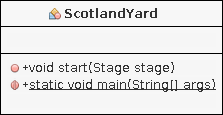
\includegraphics[scale=0.7]{img/uml/scotlandYard.png}   
            \caption{ScotlandYard UML-Klassendiagramm}
        \end{figure}


    \subsubsection{FXMLDocumentController}
        \begin{table}[H]
            \caption{Klasse FXMLDocumentController}
            \begin{tabular}{p{2.5cm}  p{9.5cm}} 
                \hline
                \textbf{Eigenschaft} & \textbf{Beschreibung}\\
                \hline
                Name & FXMLDocumentController\\
                Ort & Source-Paket \textit{gui}\\
                \hline
                Zweck &
                Wird beim Programmstart geladen. Die Klasse kennt alle Element aus der FXML-Datei.
                Führt für Interaktionen mit der GUI die entsprechenden Handler aus.
                \\
                \hline
                Beschreibung &
                \begin{itemize}
                    \itemsep0em
                    \item Instanziiert eine \textit{JavaFXGui}-Instanz und übergibt dieser alle benötigten FXML-Elemente
                    \item Instanziiert eine \textit{GameLogic}-Instanz und übergibt dieser die \textit{JavaFXGui}-Instanz
                    \item Reicht alle Interaktionen von der GUI weiter an die \textit{GameLogic} damit sie dort verarbeitet werden können
                \end{itemize}
                \\
                \hline
            \end{tabular}
        \end{table}
        \begin{figure}[H]
            \centering
            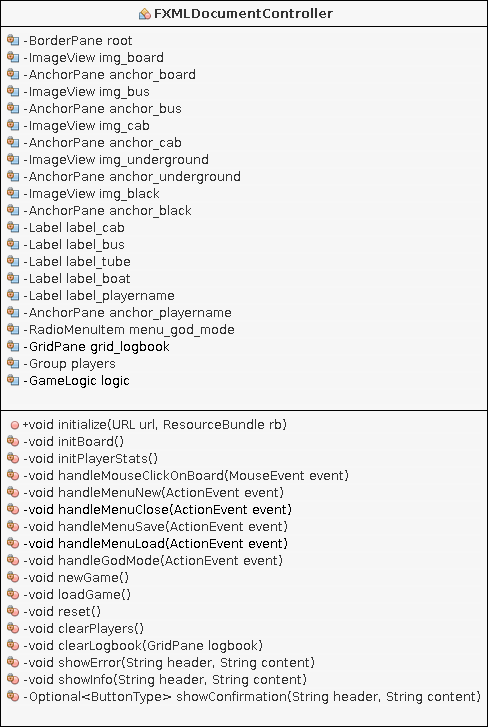
\includegraphics[scale=0.65]{img/uml/fxmlDocumentController.png}   
            \caption{FXMLDocumentController UML-Klassendiagramm}
        \end{figure}


    \subsubsection{FXMLDocument.fxml}
        Die Datei enthält alle graphischen Elemente die für das \textit{ScotlandYard} benötigt werden.
        Darunter zählen \textit{Id}'s oder auch Methoden die eine Interaktion erlauben.
        Diese Datei wird benötigt um die GUI aufzubauen und mit ihr zu interagieren.

    \subsubsection{JavaFXGui}
        \begin{table}[H]
            \caption{Klasse JavaFXGui}
            \begin{tabular}{p{2.5cm}  p{9.5cm}} 
                \hline
                \textbf{Eigenschaft} & \textbf{Beschreibung}\\
                \hline
                Name & JavaFXGui\\
                Ort & Source-Paket \textit{gui}\\
                \hline
                Zweck &
                Implementiert, das von der \textit{Logic} vorgeschriebene \textit{GUIConnector-Interface}.
                Dadurch kann die \textit{GameLogic} auf Elemente der graphischen Oberfläche zugreifen.
                \\
                \hline
                Beschreibung &
                \begin{itemize}
                    \itemsep0em
                    \item Erhält beim Instanziieren alle nötigen Elemente der graphischen Oberfläche
                    \item Implementiert Methoden zur Darstellung der Spieler und ihrer Informationen
                    \item Implementiert Methoden zur Darstellung von Dialogen und sowie Infomeldungen
                \end{itemize}
                \\
                \hline
            \end{tabular}
        \end{table}
        \begin{figure}[H]
            \centering
            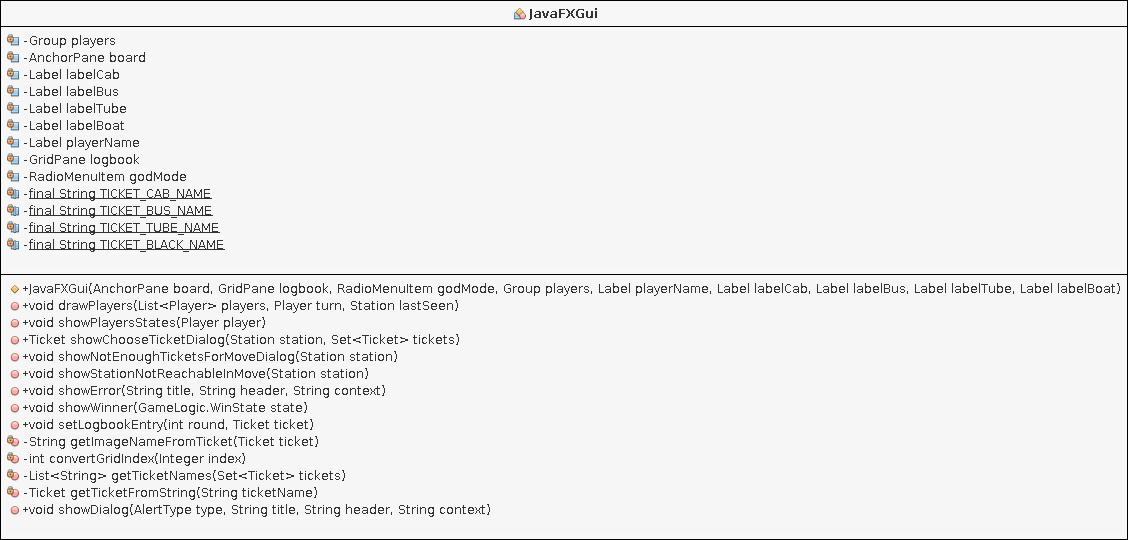
\includegraphics[scale=0.35]{img/uml/javaFXGui.png}   
            \caption{JavaFXGui UML-Klassendiagramm}
        \end{figure}



        \newpage
        \subsection{Logic-Quellpaket}
    \subsubsection{GUIConnector}
        \begin{table}[H]
            \caption{Interface GUIConnector}
            \begin{tabular}{p{2.5cm}  p{9.5cm}} 
                \hline
                \textbf{Eigenschaft} & \textbf{Beschreibung}\\
                \hline
                Name & GUIConnector\\
                Ort & Quellpaket \textit{logic}\\
                \hline
                Zweck &
                Das Interface bildet, durch vorgegebene Methoden, eine Schnittstelle zwischen der Logik und der graphischen Oberfläche.
                Die Klassen \textit{JavaFxGUI} und \textit{FakeGui} implementieren dieses Interface.
                \\
                \hline
                Struktur &
                \begin{itemize}
                    \itemsep0em
                    \item Bietet eine Schnittstelle zur Manipulation der graphischen Elemente
                    \item Fordert alle Unterklassen alle Methoden zu implementieren
                \end{itemize}
                \\
                \hline
            \end{tabular}
        \end{table}

        \begin{figure}[H]
            \centering
            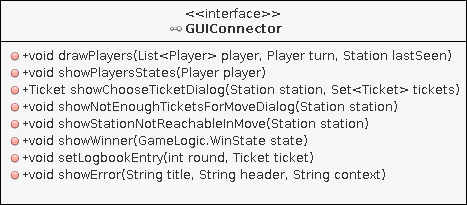
\includegraphics[scale=0.7]{img/uml/guiConnector.png}   
            \caption{GUIConnector UML-Klassendiagramm}
        \end{figure}



    \subsubsection{GameLogic}
        \begin{table}[H]
            \caption{Klasse GameLogic}
            \begin{tabular}{p{2.5cm}  p{9.5cm}} 
                \hline
                \textbf{Eigenschaft} & \textbf{Beschreibung}\\
                \hline
                Name & GameLogic\\
                Ort & Quellpaket \textit{logic}\\
                \hline
                Zweck &
                Verwaltet alle nötigen Spielelemente und lässt diese miteinander interagieren.
                Des Weiteren werden Benutzereingaben vom \textit{FXMLDocumentController}, wie ein Klicken auf ein Element in der graphischen Oberfläche,
                an die \textit{GameLogic} delegiert um dort verarbeitet zu werden.
                \\
                \hline
                Struktur &
                \begin{itemize}
                    \itemsep0em
                    \item Hält eine statische Klasse \textit{Config} in der alle wichtigen Konstanten abgelegt sind
                    \item Verwaltet das Spielfeld in einer \textit{Board}-Instanz
                    \item Verwaltet eine Gruppe an Detektiven in mehreren \textit{Detective}-Instanzen und Mister-X in einer \textit{MisterX}-Istanz
                    \item Nimmt Benutzereingaben entgegen und verarbeitet diese ihren \textit{handler}-Methoden
                    \item Ein Spiel kann über einen speziellen Konstruktor geladen werden
                    \item Regelt den Ablauf zwischen jedem Zug und steuert die KI der einzelnen Spieler
                    \item Hält zusätzliche Informationen über das Spiel wie die Spielrunde oder wer aktuell dran ist
                \end{itemize}
                \\
                \hline
            \end{tabular}
        \end{table}
        \begin{figure}[H]
            \centering
            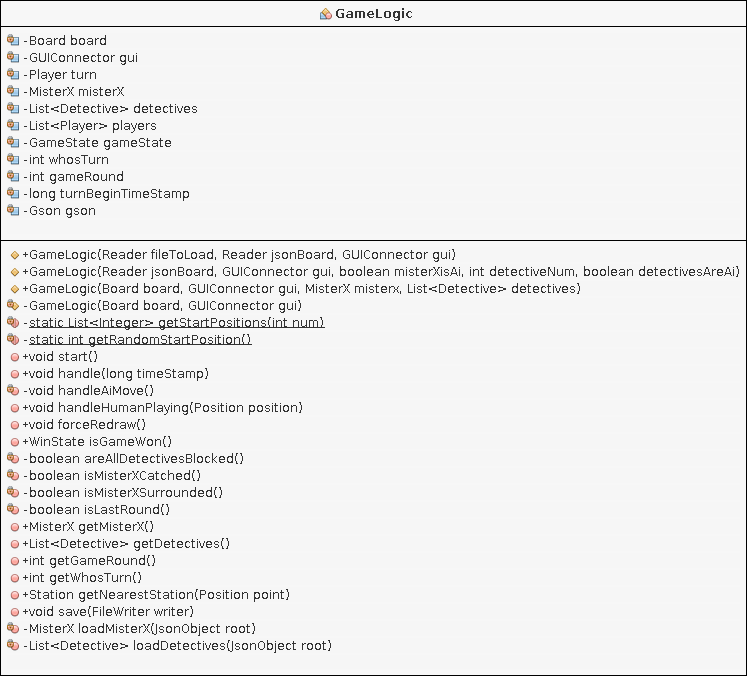
\includegraphics[scale=0.5]{img/uml/gameLogic.png}   
            \caption{GameLogic UML-Klassendiagramm}
        \end{figure}


    \subsubsection{Move}
        \begin{table}[H]
            \caption{Klasse Move}
            \begin{tabular}{p{2.5cm}  p{9.5cm}} 
                \hline
                \textbf{Eigenschaft} & \textbf{Beschreibung}\\
                \hline
                Name & Move\\
                Ort & Quellpaket \textit{logic}\\
                \hline
                Zweck &
                Repräsentiert einen Zug innerhalb des Netzes.
                \\
                \hline
                Struktur &
                \begin{itemize}
                    \itemsep0em
                    \item Hält eine \textit{Station}-Instanz die das Ziel des Zuges repräsentiert
                    \item Hält ein \textit{Ticket}-Wert der das Ticket für den Zug wiederspiegelt
                \end{itemize}
                \\
                \hline
            \end{tabular}
        \end{table}
        \begin{figure}[H]
            \centering
            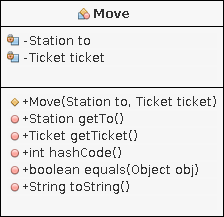
\includegraphics[scale=0.7]{img/uml/move.png}   
            \caption{Move UML-Klassendiagramm}
        \end{figure}


    \subsubsection{Ticket}
        \begin{table}[H]
            \caption{Klasse Ticket}
            \begin{tabular}{p{2.5cm}  p{9.5cm}} 
                \hline
                \textbf{Eigenschaft} & \textbf{Beschreibung}\\
                \hline
                Name & Ticket\\
                Ort & Quellpaket \textit{logic}\\
                \hline
                Zweck &
                Bildet die Tickets für die verschiedenen Verkehrsmittel ab.
                \\
                \hline
                Struktur &
                \begin{itemize}
                    \itemsep0em
                    \item Hält die Enumkonstanten \textit{CAB, BUS, TUBE, BLACK}
                    \item bietet über die \textit{from}-Methode eine Möglichkeit über einen Ordinalwert ein Ticket zu generieren
                \end{itemize}
                \\
                \hline
            \end{tabular}
        \end{table}
        \begin{figure}[H]
            \centering
            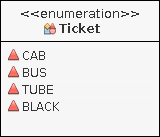
\includegraphics[scale=0.7]{img/uml/ticket.png}   
            \caption{Ticket UML-Klassendiagramm}
        \end{figure}



        \newpage
        \subsection{Logic.util-Quellpaket}
    \subsubsection{Logger}
        \begin{table}[H]
            \caption{Klasse Logger}
            \begin{tabular}{p{2.5cm}  p{9.5cm}} 
                \hline
                \textbf{Eigenschaft} & \textbf{Beschreibung}\\
                \hline
                Name & Logger\\
                Ort & Quellpaket \textit{logic.util}\\
                \hline
                Zweck &
                Die Klasse \textit{Logger} bietet die Möglichkeit Spielinformationen in einer Datei zu speichern 
                \\
                \hline
                Struktur &
                \begin{itemize}
                    \itemsep0em
                    \item Die \textit{printNewGame}-Methode speichert die generellen Informationen des Spielfeldes
                    \item Die \textit{printMove}-Methode speichert jeweils einen Zug eines Spielers
                \end{itemize}
                \\
                \hline
            \end{tabular}
        \end{table}
        \begin{figure}[H]
            \centering
            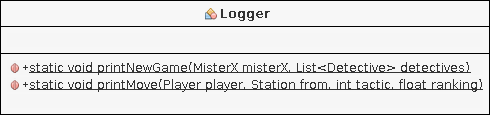
\includegraphics[scale=0.7]{img/uml/logger.png}   
            \caption{Logger UML-Klassendiagramm}
        \end{figure}


    \subsubsection{JsonValidator}
        \begin{table}[H]
            \caption{Klasse JsonValidator}
            \begin{tabular}{p{2.5cm}  p{9.5cm}} 
                \hline
                \textbf{Eigenschaft} & \textbf{Beschreibung}\\
                \hline
                Name & JsonValidator\\
                Ort & Quellpaket \textit{logic.util}\\
                \hline
                Zweck &
                Bietet Methoden zur Überprüfung der \textit{JSON}-Datenstruktur für einen Spielstand und des Netzes.
                \\
                \hline
                Struktur &
                \begin{itemize}
                    \itemsep0em
                    \item Die \textit{validateBoard}-Methode validiert die \textit{JSON}-Datenstruktur des Spielfeldes
                    \item Die \textit{validateSaveState}-Methode validiert die \textit{JSON}-Datenstruktur der Spielstandsdatei
                \end{itemize}
                \\
                \hline
            \end{tabular}
        \end{table}
        \begin{figure}[H]
            \centering
            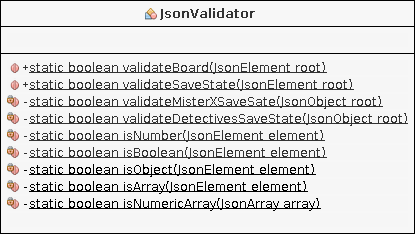
\includegraphics[scale=0.7]{img/uml/jsonValidator.png}   
            \caption{JsonValidator UML-Klassendiagramm}
        \end{figure}

    \subsubsection{GameLogicSerializer}
        \begin{table}[H]
            \caption{Klasse GameLogicSerializer}
            \begin{tabular}{p{2.5cm}  p{9.5cm}} 
                \hline
                \textbf{Eigenschaft} & \textbf{Beschreibung}\\
                \hline
                Name & GameLogicSerializer\\
                Ort & Quellpaket \textit{logic.util}\\
                \hline
                Zweck &
                Die \textit{GameLogicSerializer}-Klasse ist eine Hilfsmethode für die \textit{GSON}-Bibliothek
                und bietet einen benutzerdefinierten Serialisierer für die \textit{GameLogic}.
                \\
                \hline
                Struktur &
                \begin{itemize}
                    \itemsep0em
                    \item Wird von \textit{GSON} selbst instanziiert und verwendet.
                    Bietet über die \textit{serialize}-Methode die Möglichkeit eine \textit{GameLogic}-Instanz in ein \textit{JsonObject}
                    nach Aufgabenstellung zu transformieren.
                \end{itemize}
                \\
                \hline
            \end{tabular}
        \end{table}
        \begin{figure}[H]
            \centering
            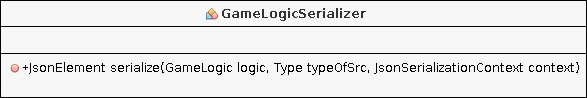
\includegraphics[scale=0.6]{img/uml/gameLogicSerializer.png}   
            \caption{GameLogicSerializer UML-Klassendiagramm}
        \end{figure}

    \subsubsection{MisterXSerializer}
        \begin{table}[H]
            \caption{Klasse MisterXSerializer}
            \begin{tabular}{p{2.5cm}  p{9.5cm}} 
                \hline
                \textbf{Eigenschaft} & \textbf{Beschreibung}\\
                \hline
                Name & MisterXSerializer\\
                Ort & Quellpaket \textit{logic.util}\\
                \hline
                Zweck &
                Die \textit{MisterXSerializer}-Klasse ist eine Hilfsmethode für die \textit{GSON}-Bibliothek
                und bietet einen benutzerdefinierten Serialisierer für \textit{MisterX}.
                \\
                \hline
                Struktur &
                \begin{itemize}
                    \itemsep0em
                    \item Wird von \textit{GSON} selbst instanziiert und verwendet.
                    Bietet über die \textit{serialize}-Methode die Möglichkeit eine \textit{MisterX}-Instanz in ein \textit{JsonObject}
                    nach Aufgabenstellung zu transformieren.
                \end{itemize}
                \\
                \hline
            \end{tabular}
        \end{table}
        \begin{figure}[H]
            \centering
            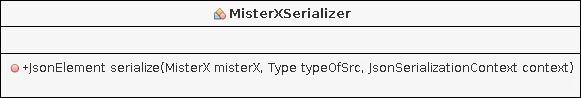
\includegraphics[scale=0.6]{img/uml/misterXSerializer.png}   
            \caption{MisterXSerializer UML-Klassendiagramm}
        \end{figure}


    \subsubsection{DetectiveSerializer}
        \begin{table}[H]
            \caption{Klasse MisterXSerializer}
            \begin{tabular}{p{2.5cm}  p{9.5cm}} 
                \hline
                \textbf{Eigenschaft} & \textbf{Beschreibung}\\
                \hline
                Name & MisterXSerializer\\
                Ort & Quellpaket \textit{logic.util}\\
                \hline
                Zweck &
                Die \textit{DetectiveSerializer}-Klasse ist eine Hilfsmethode für die \textit{GSON}-Bibliothek
                und bietet einen benutzerdefinierten Serialisierer für \textit{Detective}.
                \\
                \hline
                Struktur &
                \begin{itemize}
                    \itemsep0em
                    \item Wird von \textit{GSON} selbst instanziiert und verwendet.
                    Bietet über die \textit{serialize}-Methode die Möglichkeit eine \textit{Detective}-Instanz in ein \textit{JsonObject}
                    nach Aufgabenstellung zu transformieren.
                \end{itemize}
                \\
                \hline
            \end{tabular}
        \end{table}
        \begin{figure}[H]
            \centering
            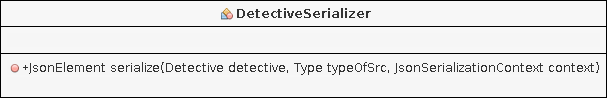
\includegraphics[scale=0.6]{img/uml/detectiveSerializer.png}   
            \caption{DetectiveSerializer UML-Klassendiagramm}
        \end{figure}


        \newpage
        \subsection{Logic.board-Quellpaket}
        \subsubsection{Board}
            \begin{table}[H]
                \caption{Klasse Board}
                \begin{tabular}{p{2.5cm}  p{9.5cm}} 
                    \hline
                    \textbf{Eigenschaft} & \textbf{Beschreibung}\\
                    \hline
                    Name & Board\\
                    Ort & Quellpaket \textit{logic.board}\\
                    \hline
                    Zweck &
                    Repräsentiert das komplette Spielfeld mit all seinen Stationen und Verbindungen.
                    \\
                    \hline
                    Struktur &
                    \begin{itemize}
                        \itemsep0em
                        \item Das Spielfeld lässt sich über eine \textit{JSON}-Datenstruktur, die das Spielfeld abbildet, laden.
                        \item Hält eine \textit{stations}-\textit{ArrayList} aus \textit{Station}-Instanzen
                        \item Die \textit{getStation}-Methode bietet die Möglichkeit eine Station über ihre Identifikationsnummer zu bekommen
                    \end{itemize}
                    \\
                    \hline
                \end{tabular}
            \end{table}
            \begin{figure}[H]
                \centering
                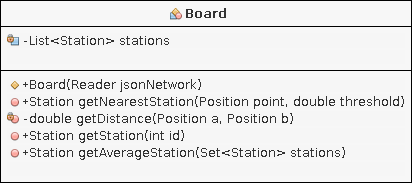
\includegraphics[scale=0.7]{img/uml/board.png}   
                \caption{Board UML-Klassendiagramm}
            \end{figure}


        \subsubsection{Station}
            \begin{table}[H]
                \caption{Klasse Station}
                \begin{tabular}{p{2.5cm}  p{9.5cm}} 
                    \hline
                    \textbf{Eigenschaft} & \textbf{Beschreibung}\\
                    \hline
                    Name & Station\\
                    Ort & Quellpaket \textit{logic.board}\\
                    \hline
                    Zweck &
                    Repräsentiert eine Station und somit einen Knotenpunkt im Netz.
                    \\
                    \hline
                    Struktur &
                    \begin{itemize}
                        \itemsep0em
                        \item Hält vier \textit{Sets} von \textit{Stations} die jeweils ein Verbindung zu anderen Stationen repräsentieren
                        \item Besitzt ein \textit{Occupied}-Flag welches aussagt, ob die Station besetzt ist oder nicht
                        \item Gibt über die \textit{getSurroundingStations}-Methode alle umliegenden Stationen zurück
                        \item Gibt über die \textit{getStationsReachableBy}-Methode alle Stationen wieder, die über das übergebene Ticket erreichbar sind
                        \item Gibt über die \textit{getTicketsToReachableStation}-methode das Ticket wieder, welches benötigt wird um die Station zu erreichen
                    \end{itemize}
                    \\
                    \hline
                \end{tabular}
            \end{table}

            \begin{figure}[H]
                \centering
                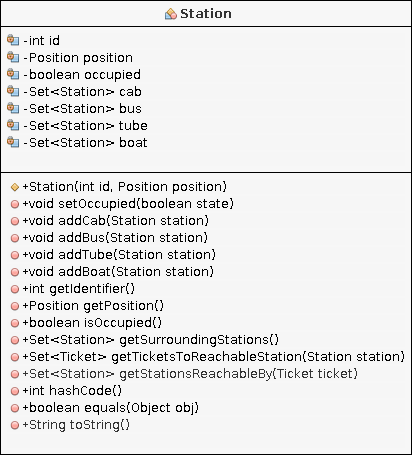
\includegraphics[scale=0.7]{img/uml/station.png}   
                \caption{Station UML-Klassendiagramm}
            \end{figure}



        \subsubsection{Position}
            \begin{table}[H]
                \caption{Klasse Position}
                \begin{tabular}{p{2.5cm}  p{9.5cm}} 
                    \hline
                    \textbf{Eigenschaft} & \textbf{Beschreibung}\\
                    \hline
                    Name & Position\\
                    Ort & Quellpaket \textit{logic.board}\\
                    \hline
                    Zweck &
                    Eine Hilfsklasse die zweidimensionale Koordinaten abbildet.
                    Wird benötigt um die Position der Stationen zu speichern.
                    \\
                    \hline
                    Struktur &
                    \begin{itemize}
                        \itemsep0em
                        \item Hält jeweils den X und den Y Anteil einer Position
                        \item bietet Funktionen die X und Y Werte auszulesen
                    \end{itemize}
                    \\
                    \hline
                \end{tabular}
            \end{table}

            \begin{figure}[H]
                \centering
                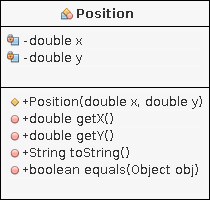
\includegraphics[scale=0.7]{img/uml/position.png}   
                \caption{Position UML-Klassendiagramm}
            \end{figure}
        \newpage
        \subsection{Logic.player-Quellpaket}
    \subsubsection{Player}
        \begin{table}[H]
            \caption{Klasse Player}
            \begin{tabular}{p{2.5cm}  p{9.5cm}} 
                \hline
                \textbf{Eigenschaft} & \textbf{Beschreibung}\\
                \hline
                Name & Player\\
                Ort & Quellpaket \textit{logic.player}\\
                \hline
                Zweck &
                Bietet eine abstrakte Oberklasse für die \textit{Detective}-Klasse und die \textit{MisterX}-Klasse
                und implementiert dabei alle grundlegenden Funktionen die benötigt werden um als
                Spieler am Spielgeschehen teilzunehmen. Darunter zählen Bewertungsfunktionen für die KI die für alle Spieler gleich sind
                oder auch die Ticketverwaltung sowie die Wegfindung.
                \\
                \hline
                Struktur &
                \begin{itemize}
                    \itemsep0em
                    \item Hält alle grundlegenden Informationen über einen Spieler wie die Tickets in dem \textit{ticket}-\textit{Array},
                        die aktuelle Station in der \textit{currentStation}-Variable als \textit{Station}-Instanz und ob der Spieler durch die KI oder 
                        durch einen menschlichen Spieler gesteuert wird in der \textit{ai}-Variable als \textit{boolean}
                    \item Die \textit{getShortestWay}-Methode bietet die Möglichkeit den kürzesten Weg durch das Netz zu finden und macht dabei
                            gebrauch von der \textit{StationDistance}-Klasse
                    \item Fordert die implementierung der \textit{play}-Methode.
                    Dadurch lässt sich die KI der Detektive und die von MisterX gleich behandeln.
                \end{itemize}
                \\
                \hline
            \end{tabular}
        \end{table}
        \begin{figure}[H]
            \centering
            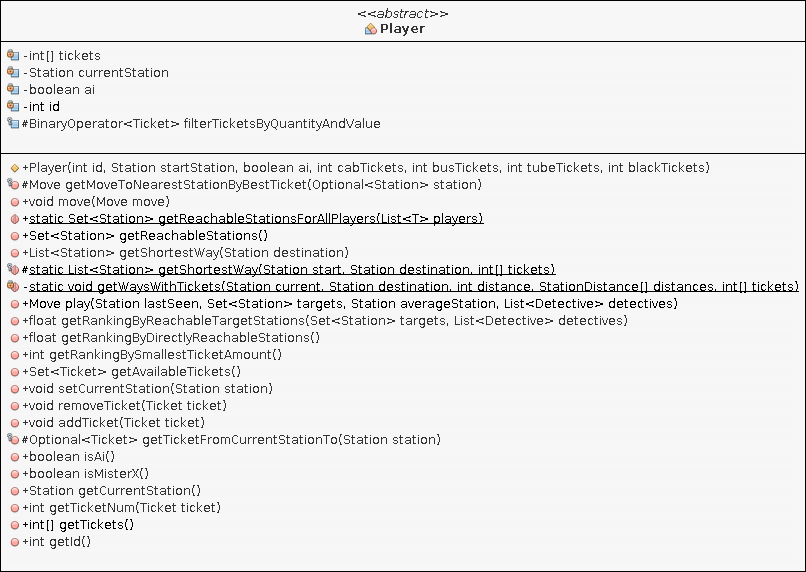
\includegraphics[scale=0.5]{img/uml/player.png}   
            \caption{Player UML-Klassendiagramm}
        \end{figure}


    \subsubsection{MisterX}
        \begin{table}[H]
            \caption{Klasse MisterX}
            \begin{tabular}{p{2.5cm}  p{9.5cm}} 
                \hline
                \textbf{Eigenschaft} & \textbf{Beschreibung}\\
                \hline
                Name & MisterX\\
                Ort & Quellpaket \textit{logic.player}\\
                \hline
                Zweck &
                Die \textit{MisterX}-Klasse erweitert die \textit{Player}-Klasse um Spezialisierungen um als Mister-X am Spielgeschehen teilzunehmen.
                Dazu gehören die Taktiken sowie die Bewertungsfunktionen und das Fahrtenbuch.
                \\
                \hline
                Struktur &
                \begin{itemize}
                    \itemsep0em
                    \item Hält in der \textit{logbook}-Variable das Fahrtenbuch welches als Liste von Tickets repräsentiert wird sowie 
                            die Station an der sich Mister-X zuletzt gezeigt hat in der \textit{lastSeen}-Variable als \textit{Station}-Instanz
                    \item Implementiert, wie von der Oberklasse vorgegeben, die \textit{play}-Methode
                    \item Macht beim vergleichen der Taktiken gebrauch von der \textit{TacticResult}-Klasse
                \end{itemize}\\
                \hline
            \end{tabular}
        \end{table}
        \begin{figure}[H]
            \centering
            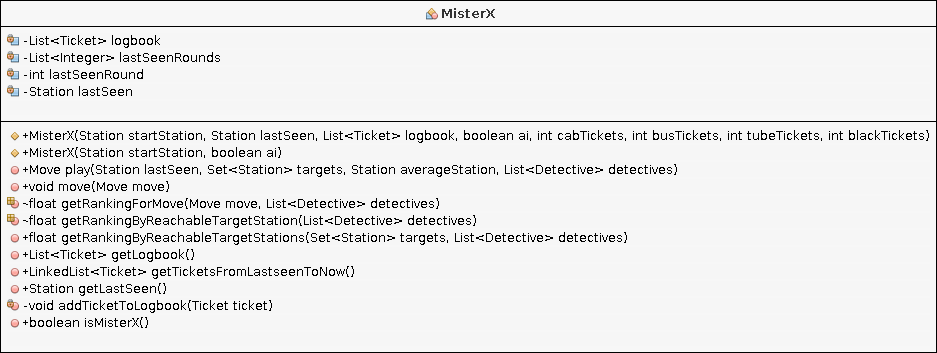
\includegraphics[scale=0.35]{img/uml/misterx.png}   
            \caption{MisterX UML-Klassendiagramm}
        \end{figure}



    \subsubsection{Detective}
        \begin{table}[H]
            \caption{Klasse Detective}
            \begin{tabular}{p{2.5cm}  p{9.5cm}} 
                \hline
                \textbf{Eigenschaft} & \textbf{Beschreibung}\\
                \hline
                Name & Detective\\
                Ort & Quellpaket \textit{logic.player}\\
                \hline
                Zweck &
                Die \textit{Detective}-Klasse erweitert die \textit{Player}-Klasse um Spezialisierungen um als Detektiv am Spielgeschehen teilzunehmen.
                Dazu gehören die Taktiken sowie die Bewertungsfunktionen
                \\
                \hline
                Struktur &
                \begin{itemize}
                    \itemsep0em
                    \item Implementiert, wie von der Oberklasse vorgegeben, die \textit{play}-Methode
                    \item Macht beim vergleichen der Taktiken gebrauch von der \textit{TacticResult}-Klasse
                \end{itemize}
                \\
                \hline
            \end{tabular}
        \end{table}
        \begin{figure}[H]
            \centering
            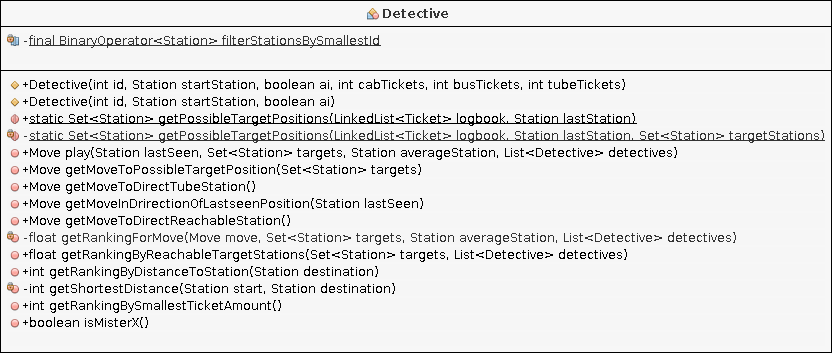
\includegraphics[scale=0.4]{img/uml/detective.png}   
            \caption{Detective UML-Klassendiagramm}
        \end{figure}


    \subsubsection{TacticResult}
        \begin{table}[H]
            \caption{Klasse TacticResult}
            \begin{tabular}{p{2.5cm}  p{9.5cm}} 
                \hline
                \textbf{Eigenschaft} & \textbf{Beschreibung}\\
                \hline
                Name & TacticResult\\
                Ort & Quellpaket \textit{logic.player}\\
                \hline
                Zweck &
                Die Hilfsklasse \textit{TacticResult} wird benötigt um die Taktiken miteinander zu vergleichen. 
                \\
                \hline
                Struktur &
                \begin{itemize}
                    \itemsep0em
                    \item Hält den Zug der Taktik als \textit{Move}-Instanz, die Identifikationsnummer und die Bewertung der Taktik.
                    \item Bietet einen Konstruktor der alle \textit{final} Attribute setzt
                    \item Bietet Getter-Methoden für die Attribute
                \end{itemize}
                \\
                \hline
            \end{tabular}
        \end{table}
        \begin{figure}[H]
            \centering
            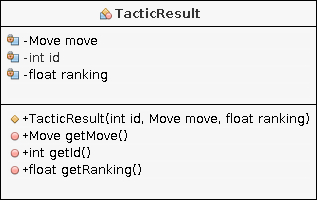
\includegraphics[scale=0.7]{img/uml/tacticResult.png}   
            \caption{TacticResult UML-Klassendiagramm}
        \end{figure}

    \subsubsection{StationDistance}
        \begin{table}[H]
            \caption{Klasse StationDistance}
            \begin{tabular}{p{2.5cm}  p{9.5cm}} 
                \hline
                \textbf{Eigenschaft} & \textbf{Beschreibung}\\
                \hline
                Name & StationDistance\\
                Ort & Quellpaket \textit{logic.player}\\
                \hline
                Zweck &
                Die Hilfsklasse \textit{StationDistance} wird für die Wegfindung benötigt und repräsentiert
                den Abstand von einer Station.
                Durch eine Menge von \textit{StationDistance} kann somit der kürzester Weg ermittelt werden. 
                \\
                \hline
                Struktur &
                \begin{itemize}
                    \itemsep0em
                    \item Hält eine \textit{Station}-Instanz welche die Station ist, die den Abstand hat der in der \textit{distance}-Variable gespeichert ist
                \end{itemize}
                \\
                \hline
            \end{tabular}
        \end{table}
        \begin{figure}[H]
            \centering
            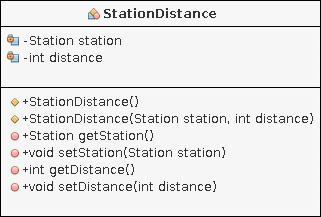
\includegraphics[scale=0.7]{img/uml/stationDistance.png}   
            \caption{StationDistance UML-Klassendiagramm}
        \end{figure}


        \newpage
        \subsection{Test.gui Quellpaket}
    \subsubsection{FakeGUI}
        \begin{table}[H]
            \caption{Klasse FakeGUI}
            \begin{tabular}{p{2.5cm}  p{9.5cm}} 
                \hline
                \textbf{Eigenschaft} & \textbf{Beschreibung}\\
                \hline
                Name & FakeGUI\\
                Ort & Quellpaket \textit{test.gui}\\
                \hline
                Zweck &
                Eine Klasse die das \textit{GUIConnector}-Interface implementiert. Dabei sind die Methoden jedoch so implementiert,
                dass diese nichts tun. So können Tests ausgeführt werden ohne ein graphische Oberfläche zu benutzen.
                \\
                \hline
                Struktur &
                \begin{itemize}
                    \itemsep0em
                    \item Alle Methoden haben einen leeren Funktionskörper
                \end{itemize}
                \\
                \hline
            \end{tabular}
        \end{table}
        \begin{figure}[H]
            \centering
            \includegraphics[scale=0.6]{img/uml/fakeGUI.png}   
            \caption{FakeGUI UML-Klassendiagramm}
        \end{figure}
        \newpage
        \subsection{Benutze Datenstrukturen}
    Die benutzen Datenstrukturen wurden in \ref{Datenstrukturen} behandelt.
   
  


    \newpage
    \section{Programmorganisationsplan}
        
Folgende Abbildung zeigt eine grundlegende Übersicht der wichtigsten Klassen und deren Zusammenwirken.
\begin{center}
    \begin{figure}[H]
        \centering
        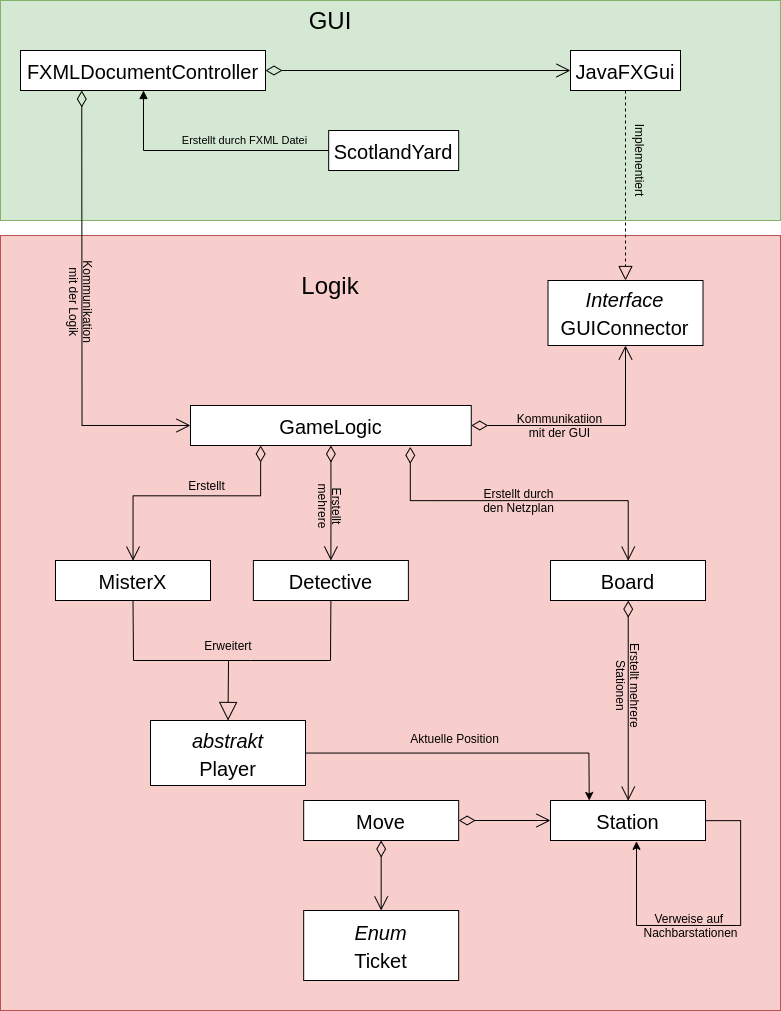
\includegraphics[scale=0.35]{img/uml/pop.png}   
        \caption{Vereinfachter Programmorganisationsplan}
    \end{figure}
\end{center}
Beim Programmstart wird die \textit{main}-Methode innerhalb der \textit{ScotlandYard}-Klasse ausgeführt.
Da die \textit{ScotlandYard}-Klasse die \textit{Application}-Klasse erweitert, wird beim aufrufen ihrer \textit{start}-Methode
die FXML-Datei geladen und daraus der \textit{FXMLDocumentController} erstellt.
Der \textit{FXMLDocumentController} besitzt alle graphischen Elemente der Oberfläche und erstellt daraus die \textit{JavaFXGui}-Klasse
und übergibt diese beim erstellen an die \textit{GameLogic}.
\newline
\newline
Die \textit{GameLogic} erstellt durch die Parameter ihres Konstruktors jeweils \textit{MisterX}, mehrere Instanzen von \textit{Detective}
und das Spielfeld (\textit{Board}). \textit{MisterX} und \textit{Detective} sind dabei Speziallisierungen der abstrakten \textit{Player}-Klasse.
Durch die übergebene \textit{JavaFXGui}-Instanz, die den \textit{GUIConnector} implementiert, kann die \textit{GameLogic} die GUI direkt manipulieren.
\newline
\newline
Das \textit{Board} erstellt beim Instanziieren alle nötigen Stationen die jeweils Referenzen auf ihre Nachbarstationen halten.
        \newpage
    \section{Programmtests}
            
    Neben den automatischen Tests kann die Logik auch mit Testdateien getestet werden.
    Diese Dateien sind speziell konstruierte Szenarien in denen ein Fehler Auftritt.
    
    \begin{table}[H]
        \caption{Spielfeld Tests}
        \begin{longtable}{p{6cm} p{4cm} p{2cm}} 
            \hline
            \textbf{Testfall} & \textbf{Erwartetes Ergebnis} & \textbf{Erzieltes Ergebnis}\\
            \hline
            Es wird getestet, ob das zu ladende Spielfeld fehlerfrei ist.
            Die entsprechenden automatischen Unit-Tests (\textit{CorruptedNetwork*}) befinden sich in \textit{GameLogicTest}.
            Manuell kann dies auch mithilfe der mitgelieferten Testdateien getestet werden.
            Dazu muss jedoch das \textit{JAR} entpackt werden und die \textit{network.json} durch die
            \textit{network\_wrongJson.json} oder die \textit{network\_wrongFormat.json} oder die
            \textit{network\_wrongValues.json} ersetzt werden. Dabei ist zu beachten, dass die ersetzende Datei in \textit{network.json}
            unbenannt werden muss. Das \textit{JAR} muss zusätzlich neu gepackt werden.
            &
            Das Programm sollte eine Fehlermeldung ausgeben, dass das zu ladende Spielfeld korrupt ist.
            &
            Das Programm gibt die Fehlermeldung aus.
            \\
            \hline
        \end{longtable}
    \end{table}

    \begin{table}[H]
        \caption{Spielstand Tests}
        \begin{longtable}{p{6cm} p{4cm} p{2cm}} 
            \hline
            \textbf{Testfall} & \textbf{Erwartetes Ergebnis} & \textbf{Erzieltes Ergebnis}\\
            \hline
            \endfirsthead
            Es wird getestet, ob die Spielstandsdatei fehlerfrei ist.
            Die entsprechenden automatischen Unit-Tests (\textit{CorruptedSaveState*}) befinden sich in \textit{GameLogicTest}.
            Manuell kann dies auch mithilfe der mitgelieferten Testdateien getestet werden.
            Dazu wird die Datei \textit{save\_wrongJson.sy} geladen um eine fehlerhafte \textit{JSON}-Struktur zu testen.
            Die Datei \textit{save\_wrongFormat.sy} hingegen testet, ob die formale Struktur eingehalten wird.
            Dies bezieht fehlende Felder mit ein.
            Die \textit{save\_wrongValues.sy} testet, ob die Werte korrekt sind. Dies beinhaltet z.B. negative Ticketanzahlen.
            &
            Das Programm sollte eine Fehlermeldung ausgeben, dass der zu ladende Spielstand korrupt ist.
            &
            Das Programm gibt die Fehlermeldung aus.
            \\
            \hline
            Es wird getestet, ob ein Spielstand erfolgreich geladen wird.
            Dazu wird die \textit{save.sy} Datei geladen.
            &
            Der Spielstand lädt erfolgreich. Dabei steht Mister-X auf der Station 138 und besitzt zehn Taxiticktes,
            acht Bustickets, 4 U-Bahntickets und 2 Blacktickets. Das Fahrtenbuch ist dabei leer.
            Die Detektive stehen jeweils auf den Stationen 197, 34 und 94 und besitzen 10 Taxitickets, 8 Bustickets und 4 U-Bahntickets.
            Mister-X ist am Zug.
            &
            der Spielstand wird erfolgreich geladen und die Werte werden korrekt angezeigt.
            \\
            \hline
        \end{longtable}
    \end{table}


    \begin{table}[H]
        \caption{Interaktions Tests}
        \begin{longtable}{p{6cm} p{4cm} p{2cm}} 
            \hline
            \textbf{Testfall} & \textbf{Erwartetes Ergebnis} & \textbf{Erzieltes Ergebnis}\\
            \hline
            \textbf{Station nicht erreichbar}\\
            Es wird getestet, ob der Fehler abgefangen wird falls ein Spieler eine Station anklickt die zu weit entfernt wird.
            Dafür wird das Spiel gestartet und auf eine Station geklickt die zu weit weg ist als, dass diese erreicht werden kann.
            &
            Das Programm sollte eine Infomeldung ausgeben, dass die Station nicht in einem Zug erreicht werden kann.
            Zudem sollte der Spieler die erneute Möglichkeit haben eine Station zu wählen.
            &
            Das Programm gibt die Infomeldung aus.
            \\
            \hline
            \textbf{Station über mehrere Tickets erreichbar}\\
            Es wird getestet, ob dem Spieler eine Möglichkeit geboten wird zwischen mehreren Tickets zu wählen, falls dieser eine Station ausgewählt hat
            die über mehrere Tickets angefahren werden kann.
            Dazu klickt der Spieler auf eine erreichbare Station die über mehrere Verbindung erreichbar ist.
            &
            Dem Spieler sollte ein Dialog gezeigt werden, sodass dieser ein Ticket auswählen kann. Steuert der Spieler Mister-X wird ihm immer das Blackticket angeboten solange
            dieser noch über genügend Blacktickets verfügt.
            Falls der Spieler über kein Ticket mehr verfügt, sodass es keine Wahlmöglichekit gibt, wird die Station angefahren und das Ticket entfernt.
            &
            Dem Spieler wird der Dialog mit den richtigen Tickets angezeigt. Falls dieser Dialog abgebrochen bzw. geschlossen wird, wird das Ticket benutzt welches ausgewählt wurde.
            \\
            \hline
            \textbf{Keine Verfügbaren Tickets mehr übrig}\\
            Es wird getestet, ob dem Spieler eine Infomeldung ausgegeben wird, wenn ein Spieler versucht ein Verkehrsmittel zu benutzen
            wofür er keine Tickets mehr hat.
            Dazu wird solange gespielt, bis von einem Verkehrsmittel keine Tickets mehr vorhanden sind.
            &
            Dem Spieler sollte eine Infomeldung angezeigt werden, dass ihm keine Tickets mehr zur Verfügung stehen.
            &
            Dem Spieler wird die Infomeldung angezeigt.
            \\
            \hline
        \end{longtable}
    \end{table}

    \begin{table}[H]
        \caption{Einstellungs Tests}
        \begin{longtable}{p{6cm} p{4cm} p{2cm}} 
            \hline
            \textbf{Testfall} & \textbf{Erwartetes Ergebnis} & \textbf{Erzieltes Ergebnis}\\
            \hline
            \endfirsthead
            \textbf{Godmode}\\
            Es wird getestet, ob der Godmode funktioniert.
            Dabei wird das Spiel gestartet und auf eine Spielsituation abgewartet, in der sich Mister-X nicht zeigt.
            Nun wird auf den \textit{Godmode}-Menüpunkt gedrückt.
            &
            Mister-X sollte sich sofort zeigen. Nach wiederholten drücken auf den Menüpunkt sollte dieser sich sofort wieder verstecken.
            &
            Mister-X wird korrekt dargestellt.
            \\
            \hline
        \end{longtable}
    \end{table}

